\documentclass{article}
\usepackage{amsmath}
\usepackage[utf8]{inputenc}
\usepackage[T1]{fontenc}
\usepackage[ngerman]{babel}
\usepackage{amsfonts}
\usepackage[left=3cm,right=2cm,top=2.5cm,bottom=2cm]{geometry}
\usepackage{karnaugh-map}
\usepackage{tikz}
\usepackage{cancel}
% \usepackage{circuitikz}
\usepackage{kvmap}
\usepackage{subcaption}
\usepackage{placeins}
\usepackage[european,noarrowmos]{circuitikz}
% \usetikzlibrary{calc,intersections,shapes.gates.logic.IEC}

\title{Grundlagen der Rechnerarchitektur: Übungsblatt 7}
\author{Alexander Waldenmaier, Maryia Masla}

\begin{document}
    \maketitle
	\subsection*{Aufgabe 1: Wiederholung: Quine McCluskey}
	\begin{enumerate}
		\item[a)] \hfill \\
		\begin{minipage}{0.5\textwidth}
			\newlength{\height}
			\setlength{\height}{2em}
			\newlength{\width}
			\setlength{\width}{3cm}
			\begin{tikzpicture}[baseline=(current bounding box.north)]
				\foreach \val[count=\i from 1, evaluate=\i as \j using int(\i+1)] in {
					$\overline{x_2 x_1 x_0}$,
					$\overline{x_2} x_1 \overline{x_0}$,
					$\overline{x_2 x_1} x_0$,
					$\overline{x_2} x_1 x_0$,
					$x_2 x_1 \overline{x_0}$,
					$x_2 x_1 x_0$
				}
				\node at(0\width, {-(\i-1)*\height})[] (A\i) {\i. \val};

				\foreach \val[count=\i from 1, evaluate=\i as \j using int(\i+1)] in {
					$\overline{x_2 x_0}$,
					$\overline{x_2 x_1}$,
					$\overline{x_2} x_1$,
					$x_1 \overline{x_0}$,
					$\overline{x_2} x_0$,
					$x_1 x_0$,
					$x_2 x_1$
				}
				\node at(1\width, {-(\i-1)*\height})[] (B\i) {\val};
				
				\foreach \val[count=\i from 1, evaluate=\i as \j using int(\i+1)] in {
					$\overline{x_2}$,
					$\overline{x_2}$,
					$x_1$,
					$x_1$
				}
				\node at(2\width, {-(\i-1)*\height})[] (C\i) {\val};

				\draw 
					(A1.east) edge (B1.west)
					(A2.east) edge (B1.west)
					(A1.east) edge (B2.west)
					(A3.east) edge (B2.west)
					(A2.east) edge (B3.west)
					(A4.east) edge (B3.west)
					(A2.east) edge (B4.west)
					(A5.east) edge (B4.west)
					(A3.east) edge (B5.west)
					(A4.east) edge (B5.west)
					(A4.east) edge (B6.west)
					(A6.east) edge (B6.west)
					(A5.east) edge (B7.west)
					(A6.east) edge (B7.west)
					
					(B1.east) edge (C1.west)
					(B5.east) edge (C1.west)
					(B2.east) edge (C2.west)
					(B3.east) edge (C2.west)
					(B3.east) edge (C3.west)
					(B7.east) edge (C3.west)
					(B4.east) edge (C4.west)
					(B6.east) edge (C4.west);

				\draw 
					(C2.south west) rectangle (C1.north east)
					(C4.south west) rectangle (C3.north east);
			\end{tikzpicture}
		\end{minipage}
		\begin{minipage}{0.5\textwidth}
			\renewcommand{\arraystretch}{1.2}
			\begin{tabular}{r|cccccc}
				 					& 1 & 2 & 3 & 4 & 5 & 6 \\ \hline
				$\overline{x_2}$	& + & + & + & + &   &   \\
				$x_1$				&   & + &   & + & + & +
			\end{tabular}\\ \vspace*{1cm} \\
			$\Rightarrow f(x_2, x_1, x_0) = \overline{x_2} + x_1$
		\end{minipage}
		\item[b)]
		Gatterschaltung:\\
		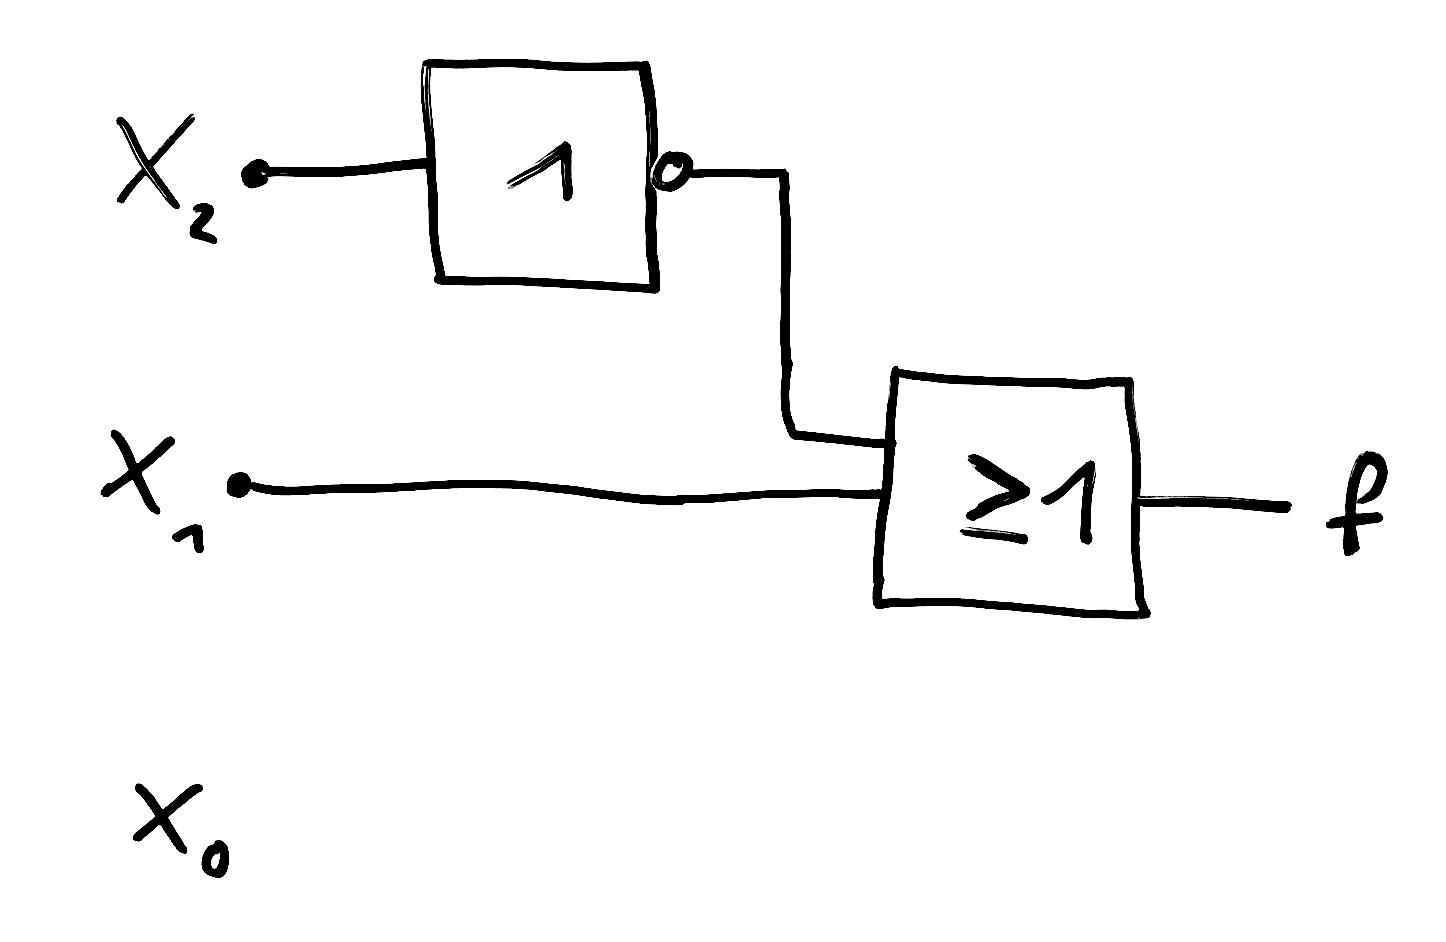
\includegraphics[width=0.3\linewidth]{aufgabe1.png}
	\end{enumerate}


	\subsection*{Aufgabe 2: Schieberegister und Asynchronzähler}
	\begin{enumerate}
		\item[a)] 4-bit FIFO-Schieberegister: \\
		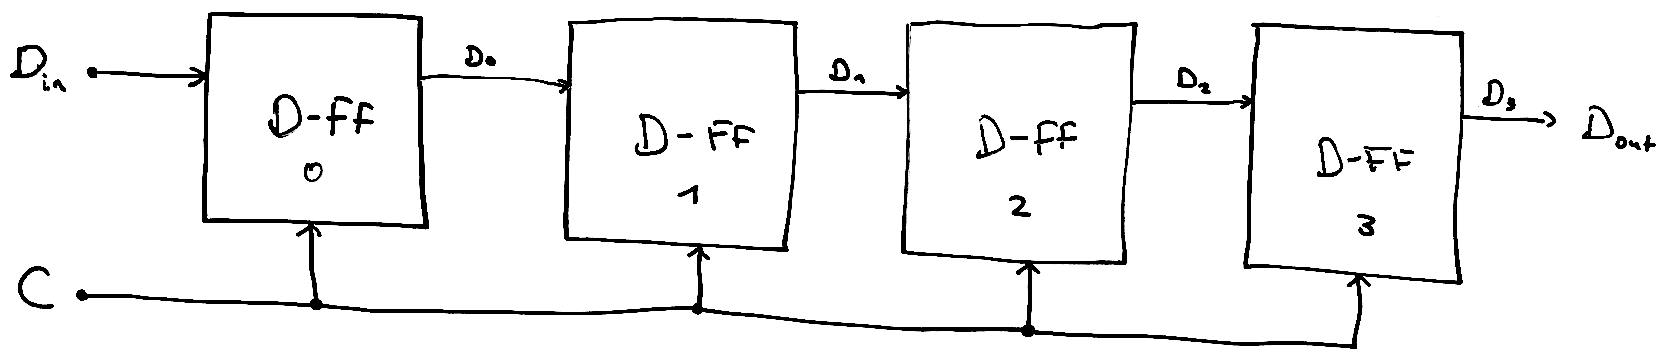
\includegraphics[width=\linewidth]{fifo_schieberegister.png}
	\end{enumerate}


	\newpage
	\subsection*{Aufgabe 4: Ripple-Carry-Addierer}
	\hfill \\
	\begin{minipage}[t]{0.02\linewidth}
		\hfill
	\end{minipage}
	\begin{minipage}[t]{0.2\linewidth}
		a) Halbaddierer: \\\\
		\begin{tabular}{cc|cc}
			$a$ & $b$ & $c_{out}$ & $s$ \\ \hline
			0 & 0 & 0 & 0 \\
			0 & 1 & 0 & 1 \\
			1 & 0 & 0 & 1 \\
			1 & 1 & 1 & 0 
		\end{tabular}
		\begin{align*}
			s(a,b) &= a \oplus b \\
			c_{out}(a,b) &= ab
		\end{align*}
	\end{minipage} 
	\begin{minipage}[t]{0.2\linewidth}
		\vspace*{1em}
		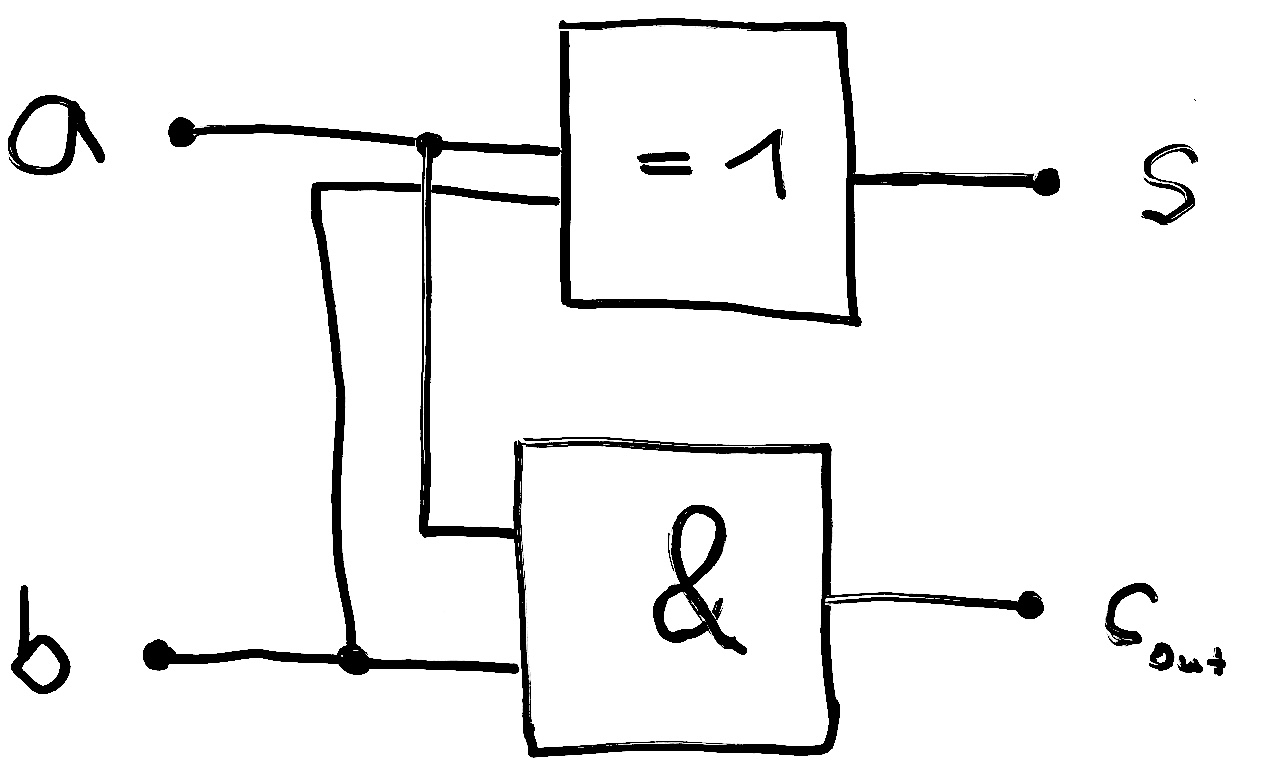
\includegraphics[width=\linewidth]{halfadder.jpeg}
	\end{minipage}
	\begin{minipage}[t]{0.1\linewidth}
		\hfill
	\end{minipage}
	\begin{minipage}[t]{0.3\linewidth}
		b) Volladdierer:\\
		\hspace{1em}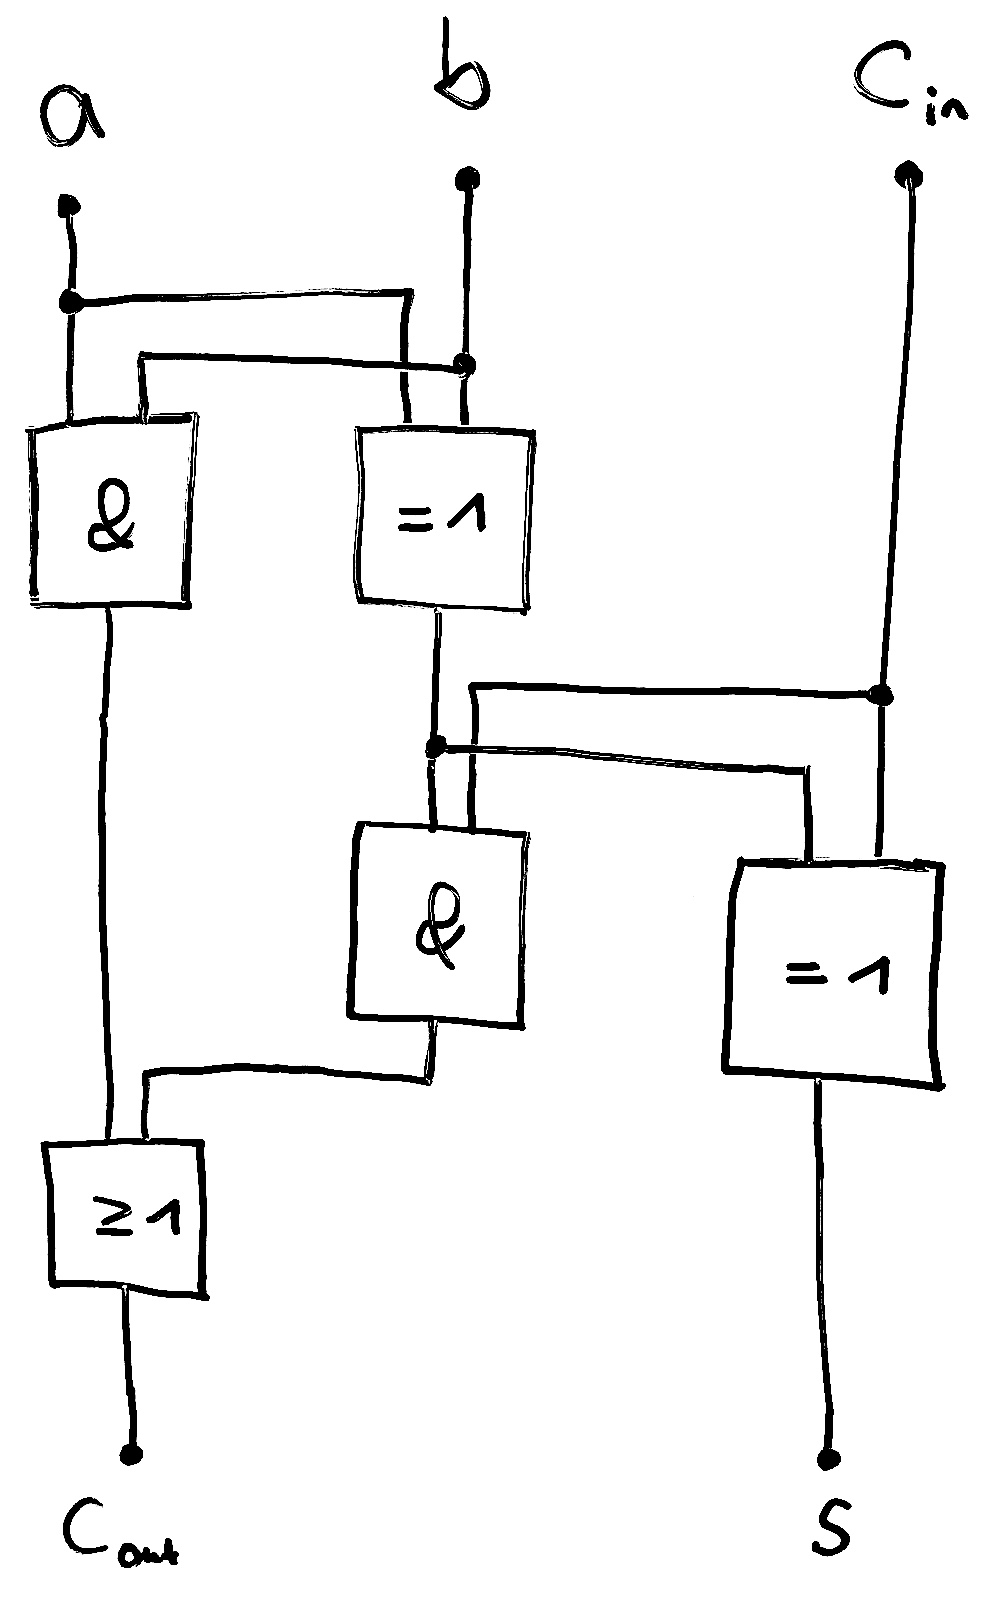
\includegraphics[width=0.8\linewidth]{fulladder.jpeg} 
	\end{minipage}
	\begin{enumerate}
		\item[c)]Ripple-Carry-Addierer:
		\begin{center}
			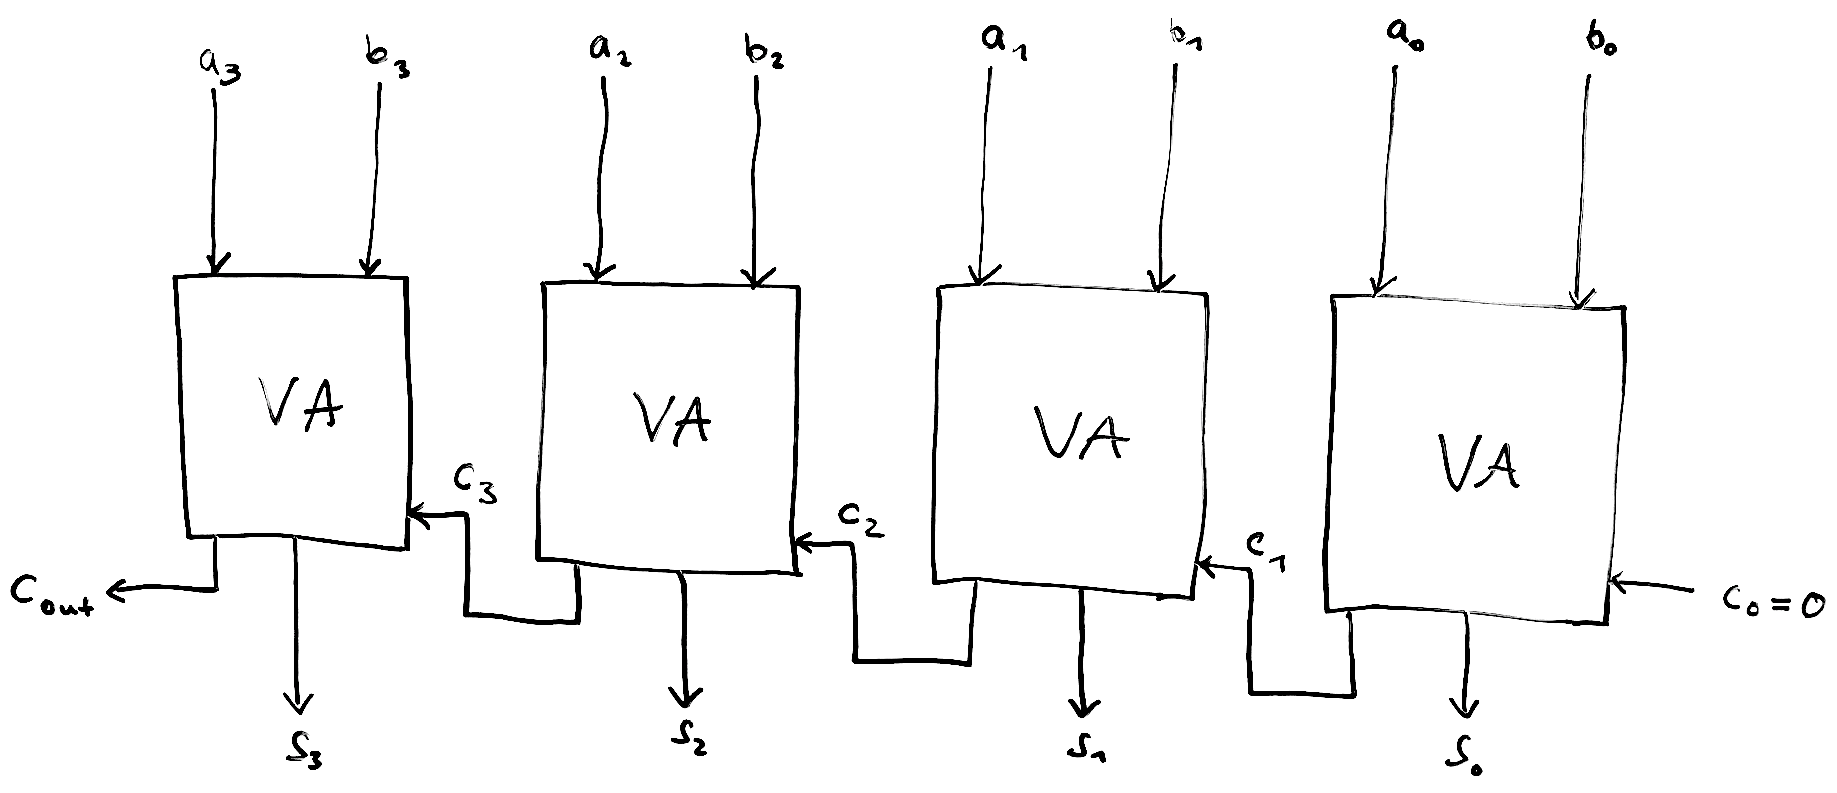
\includegraphics[width=0.8\linewidth]{ripplecarry.png} 
		\end{center}
		\item[d)]Ripple-Carry-Addierer/Subtrahierer:
		\begin{center}
			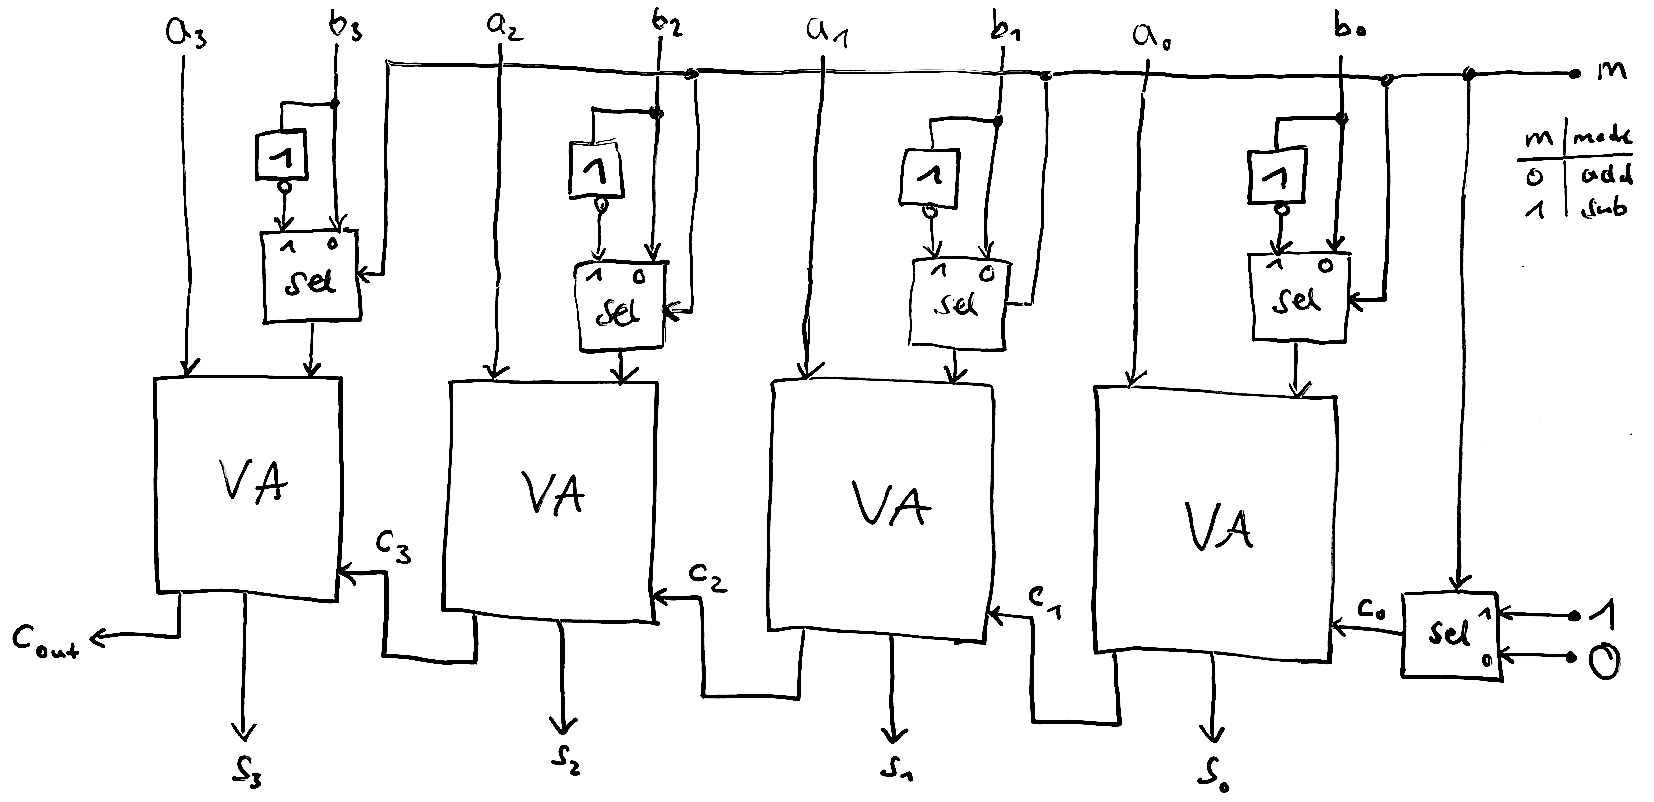
\includegraphics[width=0.9\linewidth]{carry_add_sub.jpeg}
		\end{center}
		\textit{Noch einfachere Möglichkeit: Alle Multiplexer (mit Invertern) jeweils durch XOR-Gatter ersetzen.}
		\item[e)] Der Name "`Ripple"'-Carry suggeriert bereits, dass die Carry-Information wie eine Welle der Reihe nach durch alle Volladdierer hindurchläuft. Dadurch entsteht eine besonders große Schaltungstiefe und folglich eine deutliche Restriktion auf die mögliche Taktfrequenz. 
		
		Beim Carry-Select-Addierer werden hingegen für jedes Bit beide Möglichkeiten "`durchgespielt"': Einmal mit Carry, einmal ohne. Dahintergeschaltete Multiplexer wählen dann, abhängig des Ergebnisses des vorigen Volladdierers, für das jeweilige Bit den richtigen Wert aus. Zwar muss auch hier darauf gewartet werden, bis sich der Carry durch alle Multiplexer durchpropagiert hat, allerdings geschieht dies deutlich schneller als das Durchlaufen jedes ganzen Volladdierers. Der entscheidene Nachteil: Es werden doppelt so viele Volladdierer benötigt und dazu noch die Multiplexer. 
	\end{enumerate}
\end{document}